\section{Methods}
\label{section:p450/methods}

\begin{figure}[h!]
\centering
\includegraphics[width=0.55\textwidth]{dot_files/idsite.png}
\caption{An overview of the entire IDSite procedure.
The dotted lines represent abbreviated versions of the full procedure.
Receiver operating characteristic graphs for the full version, and these abbreviated versions, are presented in \ref{figure:idsite_roc_sampling}.
Series colors on ROC graphs correspond to arrow colors here.}
\label{figure:idsite_overview}
\end{figure}

Prediction of sites of metabolism is a three stage procedure:
\begin{enumerate}
\item Initially a number of different ligand conformations are generated, and these are docked into a rigid protein, with soft VDW terms using Glide \cite{halgren2004glide,friesner2004glide}.
\item The docked conformations are refined using a Monte Carlo Minimization (MMC) approach which samples degrees of freedom in both the ligand and protein.
\item Refined conformations are classified into reactive site or non-reactive site on the basis of the energy of the refined conformations and the intrinsic reactivity of the site. \cite{li2011idsite}
\end{enumerate}

\subsection{Docking}
\label{subsection:p450/docking}
In the initial docking stage of the IDSite protocol Glide is used to generate a number of proposed docked conformations for each ligand.
Glide (standard precision) is used to generate a number of different ligand conformations by sampling conformations of freely rotatable bonds and rings.
A bounding box, which will be used for a grid search, is defined centered at the centroid of the ligand with an edge length of 10 angstroms.
Because the crystal structure used for CYP2D6 (PDBID: 2F9Q) does not have a ligand, the centroid of residues Glu216, Asp301, Thr309, and Phe483 was used instead in this case.
Because the steric clashes present in many proposed docked conformations can be relieved using a simple minimization procedure a reduced Van der Waals (VDW) radii are used in the docking stage for non-polar atoms.
The VDW radii used for the P450 are scaled by a factor of 0.4, and the scaling for the ligand starts at 0.8.
If an insufficient number of poses, in this case fewer than four, are found using these scaling factors for the radii the scaling of the ligand is stepped down until at least four poses are found.
Additional filtering of possible high energy conformations was also skipped in order to ensure the greatest diversity of docked poses reached the refinement stage.
The collection of docked poses are then clustered according to the RMSD of the ligand, and each pose is minimized.
The top sixty ranked poses according to the Glide SP metric are retained screened using a number of different criteria.
A hard sphere overlap criteria is used to remove poses with obvious steric clashes which were not removed during the minimization procedure.
A conserved feature of CYP2D6 ligand complexes is a salt bridge with Glu216 or Asp301.
In order to reduce sampling cost IDSite only considers structures with at least one hydrogen-bond donor within 4 residues of the centroid of these two residues and Ser304.
The sphere defined by these residues is illustrated along with the bounding box used for sampling in Figure \ref{fig:idsite_glide}
A number of other rule based geometric screens are used to remove structures which are unlikely to react.
Structures meeting any of the following criteria:
\begin{enumerate}
\item The distance of the basic nitrogen to the ferryl oxygen is less than 5.0 angstroms;
\item The distance of the basic nitrogen to the negative charged oxygen (in Glu216 or Asp301) is greater than 5.5 angstroms;
\item More than 2 heavy atoms from the ligands are further than 16.0 angstroms away from the heme iron;
\item More than 1 heavy atom from the ligand are closer than 1.0 angstroms to the receptor;
\item More than 6 heavy atoms from the ligand are closer than 1.8 angstroms to the receptor;
\item No heavy atom in the ligand is within 5.0 angstroms to the heme iron;
\end{enumerate}
are removed.
If the number of structures at this point is too low, the VDW scaling factors of the non-polar atoms of the ligand are stepped down, and the process is repeated.
If four or more poses are found at these point these poses are passed onto the next stage of the IDSite procedure, the Monte Carlo Minimization refinement stage.

\begin{figure}[h]
\centering
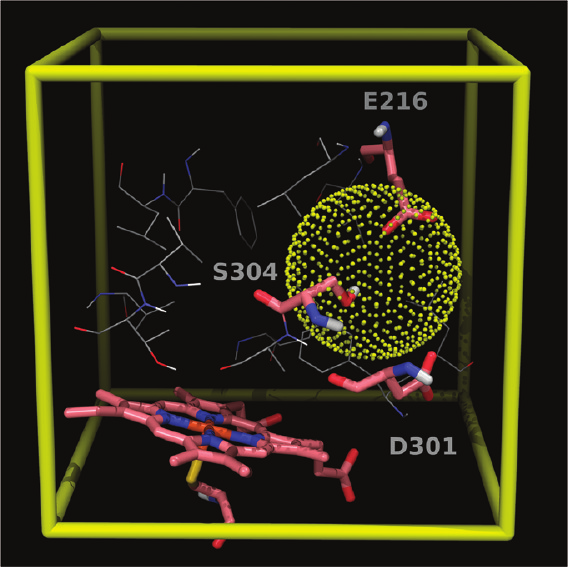
\includegraphics[width=0.35\textwidth]{figures/idsite/glide.png}
\caption{An overview of the entire IDSite procedure.}
\label{fig:idsite_glide}
\end{figure}

% IDSite uses reduced VDW radii for nonpolar atoms both in the protein receptor and the ligand, so that slight steric clashes are tolerated during the docking stage.
% For the protein receptor the VDW scaling factor is fixed at 0.40, while for the ligand, the scaling factor starting from 0.80 is adaptively adjusted until at least 4 valid poses are found.
% With highly flexible ligands and relatively high scaling factors, Glide often finds only a handful of valid poses, and even fewer survive after IDSite screening.
% However, if the scaling factor is set too low, the docked poses may contain too many serious steric clashes, which can cause problems in the subsequent minimization.
% If IDSite fails to find enough valid poses, the scaling factor is adjusted and the number of poses to pass the initial docking phase in Glide is increased accordingly to augment sampling.

% joe is this far
% If the ligand contains other hydrogen-bond donors except for the basic nitrogen, the constrained docking is likely to generate poses that form hydrogen bonds instead of the salt bridge to Glu216 or Asp301.
% However, IDSite is able to distinguish these poses and filter them via an additional salt bridge filter in the pose screening, so that only the poses with a stable salt bridge are allowed to pass to the refinement stage.


\subsection{Monte Carlo Minimization Refinement}
\label{subsection:p450/mcm}
Since the emphasis in IDSite sampling is efficient sampling of low energy conformations, as only the lowest energy conformations are passed on to the next stage of prediction, Monte Carlo Minimization, which provides more efficient sampling of low energy conformations, was used instead of a more traditional Monte Carlo simulation (see \ref{subsection:monte_carlo}).
The Monte Carlo Minimization sampling used by IDSite for refinement incorporates three different types of steps: side chain motions, rigid body transformations, and hybrid Monte Carlo simulations.
For each Monte Carlo step one of three types of motions is selected according to the weighted probabilities, which are different for the two different PLOP sampling stages, see Table \ref{table:mmc_params}.
\begin{table}[h]
    \centering
    \begin{tabular}{|c|c|c|}
        \cline{2-3}
        \multicolumn{1}{r|}{~}                       & \multicolumn{2}{c|}{PLOP Sampling Stage} \\
        \cline{2-3}
        \multicolumn{1}{r|}{~}                       & First                        & Second                        \\
        \hline
        Number of Residues Sampled                   & 12                           & 40                            \\
        \vspace{-1.5ex}
        Number of Structures                         & \multirow{2}{*}{max(n*8,24)} & \multirow{2}{*}{max(n*20,60)} \\
        Advanced to Next Stage                       &                              &                               \\
        P(side chain step)                           & 0.5                          & 0.7                           \\
        P(rigid body step)                           & 0.1                          & 0.2                           \\
        P(HMC)                                       & 0.4                          & 0.2                           \\
        \hline
    \end{tabular}
    \caption{The number of residues sampled as well as the number of structures advanced to the next stage from each of the sampling stages.
Also, the relative probabilities of selecting each of the different sampling steps during a Monte Carlo minimization sampling stage.}
    \label{table:mmc_params}
\end{table}

Using the chosen method a new conformation is proposed and minimized before the Metropolis acceptance criteria (equation \ref{equation:metropolis_acceptance}) is applied to the proposed state, using a temperature of 300 K.
All atoms of all residues with any atom within 5 Angstroms of the ligand in the starting crystal structure were allowed to move during Monte Carlo moves, including the ligand itself.

During the minimization Monte Carlo sampling stages of the IDSite procedure artificial constraints are used to guide the sampling towards a transition state like conformation.
These constraints create artificial bond or angle potentials which affect the minimization, but are not used in the Monte Carlo acceptance test.
For each of the minimization Monte Carlo sampling stages of the IDSite procedure two different sets of constraints are applied depending on the hybridization of the carbon atom at the possible site of metabolism, for a total of four possible different sets of constraints.
In the first minimization Monte Carlo stage two constraints are applied:
\begin{enumerate}
\item The sulfur-iron-carbon angle is constrained to 145 degrees, with 20 degrees of ``slack'', or a flat bottom to the potential well.
The spring constant of this constraint is about 25 kcal/mol/degree\superscript{2}, or {\textapprox}40\% the strength of a carbon-carbon-carbon angle.
\item A ``dummy'' oxygen atom is placed above the plane of the heme group, in the same position that it would occupy if an oxygen molecule was bound to the heme.  
This dummy atom has no interactions with other atoms, but is used as the anchor of a distance constraint for the carbon at the site of metabolism.  
The carbon-dummy oxygen distance is constrained to 2.5 angstroms, with 0.5 angstroms of slack.
The spring constant of this constraint is 100 kcal/mol/angstrom\superscript{2}, approximately 1/3rd the strength of a carbon-carbon bond.
\end{enumerate}
\begin{figure}[hp]
\centering
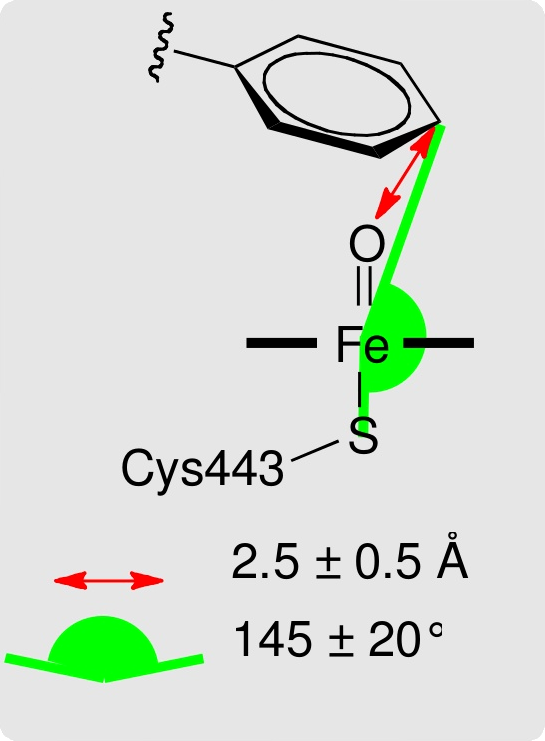
\includegraphics[width=0.25\textwidth]{figures/idsite/33b}
\caption{The constraints applied to sp\superscript{2} atoms during the constrained minimization and first minimization Monte Carlo sampling stage.
The spring constant of the bond constraint (red arrow) is 100 kcal/mol/angstrom\superscript{2}, and that of the angle constraint is 25 kcal/mol/degree\superscript{2}.
The oxygen atom depicted in this figure is a ``dummy'' atom and does not interact with any other atoms in the structure except through the constraint.}
\label{figure:first_sp2_constraints}
\end{figure}
 % figure
\begin{figure}[hp]
\centering
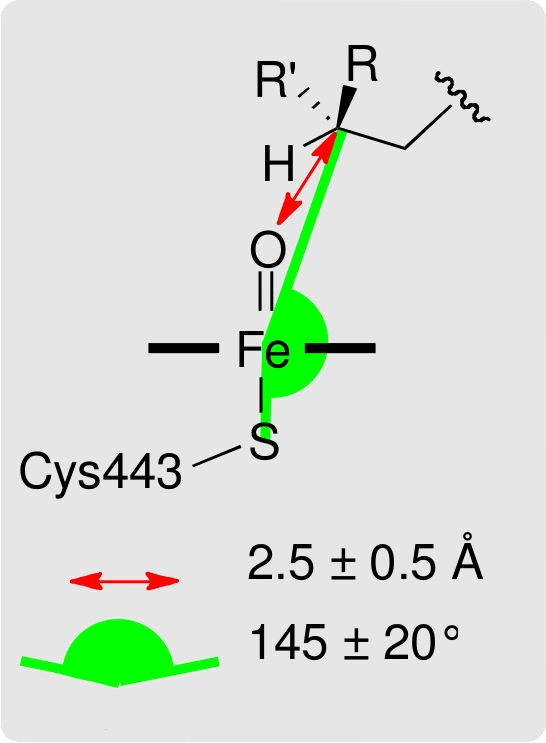
\includegraphics[width=0.25\textwidth]{figures/idsite/33a}
\caption{The constraints applied to sp\superscript{3} atoms during the constrained minimization and first minimization Monte Carlo sampling stage.
The spring constant of the bond constraint (red arrow) is 100 kcal/mol/angstrom\superscript{2}, and that of the angle constraint is 25 kcal/mol/degree\superscript{2}.
The oxygen atom depicted in this figure is a ``dummy'' atom and does not interact with any other atoms in the structure except through the constraint.}
\label{figure:first_sp3_constraints}
\end{figure}
 % figure

In the second minimization Monte Carlo sampling stage the constraints are different for sp\superscript{2} and sp\superscript{3} carbons.
For sp\superscript{3} sites:
\begin{enumerate}
\item the hydrogen bound to the carbon at the possible site of metabolism is constrained to a distance of 1.25 angstroms from the dummy oxygen atom, with 0.1 angstroms slack and a spring constant of 20 kcal/mol/angstrom\superscript{2},
\item the carbon in question is constrained to 2.2 angstroms from the heme iron, with 0.8 angstroms slack and a spring constant of 10 kcal/mol/angstrom\superscript{2},
\item the heme iron-hydrogen-carbon angle is constrained to 138 degrees, with 5 degrees slack and a spring constant of 20 kcal/mol/degree\superscript{2}.
\end{enumerate}
For sp\superscript{2} sites:
\begin{enumerate}
\item the carbon at the possible site of metabolism is constrained to 1.8 angstroms from the dummy oxygen atom, with 0.1 angstroms slack and a spring constant of 20 kcal/mol/angstrom\superscript{2},
\item both adjacent carbons are also constrained to the dummy oxygen atom, at a distance of 2.5 angstroms, with 0.1 angstroms slack and a spring constant of 20 kcal/mol/angstrom\superscript{2}, and
\item finally the hydrogen bonded to the carbon at the possible site of metabolism is constrained to the oxygen atom at a distance of 2.0 angstroms, with 0.1 angstroms slack and a 20 kcal/mol/angstrom\superscript{2} spring constant.
\end{enumerate}
\begin{figure}[hp]
\centering
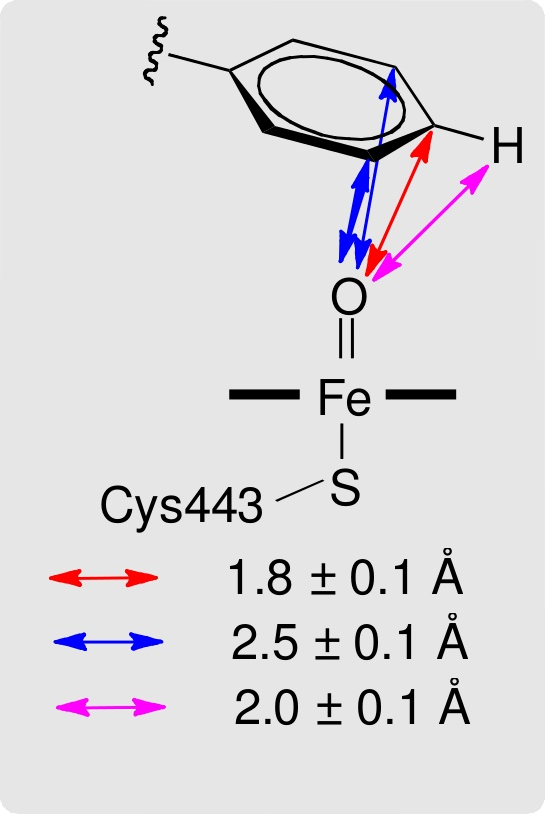
\includegraphics[width=0.25\textwidth]{figures/idsite/34b}
\caption{The constraints applied to sp\superscript{2} atoms during the constrained minimization and second minimization Monte Carlo sampling stage.}
\label{figure:second_sp2_constraints}
\end{figure}
 % figure
\begin{figure}[hp]
\centering
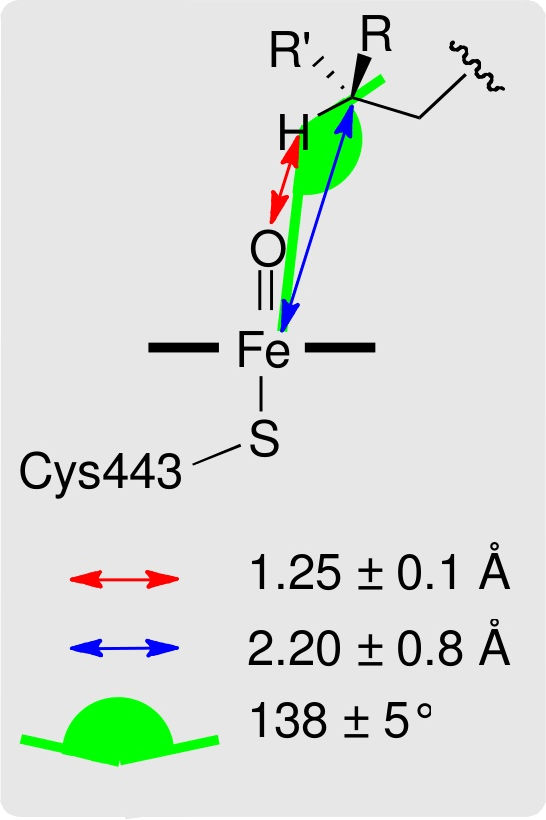
\includegraphics[width=0.25\textwidth]{figures/idsite/34a}
\caption{The constraints applied to sp\superscript{3} atoms during the constrained minimization and second minimization Monte Carlo sampling stage.}
\label{figure:second_sp3_constraints}
\end{figure}
 % figure

A separate set of constraints apply to the region containing the conserved salt bridge.

\begin{enumerate}
\item Side chain moves.
Several types of side chain motions were implemented in PLOP.
In all cases, they are defined in a such a way that they can be applied to both ligands and proteins.
The same atomic overlap screening function implemented with the rigid body Monte Carlo was implemented with the side chain torsional moves.
a. Random torsion angle moves: The first type of move that was implemented is random movement of torsional chi angles.
For small torsion moves, a random perturbation of the angle of +/- X is made, where X is a random number with user defined magnitude.
For large torsion moves, for each torsion angle that is changed, a random angle is selected in the form 60*Y +/- X, where Y = 1 through 5, and X is the same random number for the small torsion moves.
The large move was introduced since positions at the top of rotamer barriers are relatively unlikely to be selected, and efficiency thus can be improved by focusing on the more probable moves.
The ratio of small to large torsion moves can be used-adjusted, as can the ratio of probabilities of changing all the torsions in a randomly selected side chain versus changing only one single (randomly selected) torsion among all the free torsions in the simulation can be set as a user-defined parameter.
Rotamer side chain moves: A second type of torsional samples implemented is random selection of a new rotamer state for the entire side chain, plus an optional user defined small noise term for each torsion in the rotamer state.
A database of protein rotamer states obtained from crystallographic data are already a part of PLOP \cite{xiang2001extending} Rotamer libraries for ligands are generated by examining all possible side chain conformations at 10 degree resolution and screening this set for steric clashes.
A Monte Carlo move in this case represents a choice of a new torsional rotamer state for the entire side chain.
Monte Carlo moves based on torsional states cannot lead to correct equilibrium distributions, as transitions from non-rotamer states to rotamer states are defined, but not reverse transitions, upsetting detailed balance.
However, a pretabulated rotamer state is more likely to be low energy than a randomly generated torsional state, and thus allows for more diverse conformational searching.
Correlated torsional moves: Most torsional rearrangements of the side chains in the core of proteins are highly correlated because of the density.
In order to attempt to include correlated torsional motion, at each step we examine the distance between all pairs of beta carbons in the ligands that are free to move.
At each step, for the set of side chains that are free to move, clusters where beta carbons are all mutually within a user-specified distance are identified.
This process takes a trivial amount of time compared to an energy evaluation, so does not slow the simulation at all.
Then, with user specified probabilities, clusters of different sizes are selected for the torsional moves, either with random side chain moves, or rotamer selection moves.
By selecting only clusters where all residues are mutual neighbors, detailed balanced is observed for simulations where accurate equilibrium sampling is desired.
By varying the dihedral angles of the rotatable bonds, IDSite uses side chain MC moves in PLOP to sample the selected side-chain conformations of the protein and of the ligand.
Up to three close residues (C beta distance within 6 angstroms) are allowed to rotate collectively, but the moves of the protein residues and those of the ligand are separated.
In each attempted movement, the conformations of the selected side chains (from the protein/ligand) are either changed by random perturbations or assigned by the randomly selected rotamers from a library.
For an attempt with a random perturbation, the displacement of each dihedral angle is the sum of a large rotation (N times 60 degrees with N as a random integer between 0 and 5) and a random perturbation from 0 to 30 degrees.
For a rotamer library attempt, a side-chain conformation is updated with a random rotamer from a high resolution side-chain library for protein residues \cite{xiang2001extending}, and from a homogeneous library at 10 degree resolution for the ligand.
If a structure with tolerable overlaps is generated in an attempt, it is minimized and sent to subsequent stages for judgment of acceptance.
Each side-chain move takes less than 15 seconds and is the fastest among all the three move types.

% from mike's
For side chain Monte Carlo, a steric screen with an overlap factor of 0.6 was used.
Rotamer torsional moves were selected 75\% of the time, with half of the remaining being of random torsions, and the other half random perturbations of all torsions within the randomly selected side chains.
Clusters of size 1 (i.e. single side chains), size 2 and size three were selected in equal proportion, and all side chains in the cluster were perturbed with the selected torsion move.
A mutual beta carbon distance of 6 Angstroms was used for the clustering size.
Small torsion perturbations made +/- 60 degress from the current dihedral angle, and were performed 5\% of the time; Large periodic moves were performed 95\% of the time.
Only outer steps were performed, and each side chain Monte Carlo series consisted in only one move.
Minimization was performed after the single step, and acceptance was performed at 1 K.


\begin{figure}[hp]
\centering
\includegraphics[width=0.7\textwidth]{dot_files/mcm_flowchart.png}
\caption{An outline of the Monte Carlo minimization refinement stages in PLOP.}
\label{figure:mcm_flowchart}
\end{figure}
\item % TODO
Rigid motion moves.
Rigid body translation and rotation were also implemented for noncovalently linked moieties, such as ligands.
Random rotations and translations were coupled together, allowing for more concerted movement.
Rigid body move implemented in PLOP can optionally include a screening step, where atomic Lennard-Jones overlaps that would lead to energies much higher than would be observed in any conceivably long equilibrium simulation are rejected without further evaluation.
A ratio of 0.7 between the distance between the two atoms and the sum of the Lennard-Jones radii of the two atoms yields energies on the order of 10's of thousands of kcal/mol, and is thus reasonable to maintain equilibrium sampling in a Monte Carlo simulation.
Translations were implemented in a random direction, with a user-defined magnitude.
Rotations were implemented by picking a random quarternion (a random angle around a random axis, through the geometric center of the rigid group) with a user specified maximum random angle centered around either the current angle, or 180 from the current angle, in the case of a flip.
Multiple time scale Monte Carlo sampling was also implemented with rigid body moves, with short range and long range interactions defined as above.
In addition, an option to compute the inner Monte Carlo loops with reduced Lennard-Jones radii were also implemented, to increase the ability to escape from tight spacial bottlenecks.
In this case, the long time step energies are the full energies with unscaled Lennard-Jones radii.
This increases the conformational freedom and therefore sampling for the short, at a cost of decreasing the acceptance probability in the outer loop.
Scaled Lennard-Jones radii were also implemented in multiple time dynamics, but yielded very little apparent improvement because of the lack of phase space overlap between dynamics with different scaled Lennard-Jones radii).
Rigid body moves are used to sample the translational and rotational space of the ligand.
Multiple attempts with reduced VDW radii are applied, as it is quite common to fail in searching for a clash-free conformation in a single rigid body moving attempt (especially when the ligand is large and flexible and the binding pocket is relatively small).
Each rigid body move includes 1000 attempts, and each attempt performs a translation along a random vector and a rotation around a random axis, with less than 0.5 angstroms and 60 degree displacement, respectively.
In addition, the VDW radii are reduced (scaling factor 0.8) to soften the Lennard-Jones potential, so that mild steric clashes are allowed, which are likely to be resolved by the subsequent minimization.
The rigid body move usually takes 20 to 40 seconds per move.

% from mike's
For rigid body Monte Carlo, a steric screen with an overlap factor of 0.7 was used, with a translation size of 0.5 Angstroms and a rotation size of plus or minus 60 degrees.
No flip moves were included, as flips were not anticipated with the geometry of the ligand system [Robert, check this is true?] A Lennard-Jones scaling parameter of 0.8 was used during the inner steps.
Each rigid MC step consisted of 1000 inner steps, and only one outer step, meaning that only one minimization occurred each time rigid body Monte Carlo was selected as the move step.


\item The Hybrid Monte Carlo (HMC) \cite{duane1987hybrid} step is a velocity verlet molecular dynamics simulation.
This simulation allows all atoms in both the ligand and residues containing atoms withing 5 angstroms of the ligand to move.
Initial velocities are taken from a Maxwell-Boltzmann distribution at 900 K.
Bonded and short range interactions evaluated every 1 nanosecond inner time step, and long range potentials are assumed to be fixed over inner steps.
Five inner steps compose each outer HMC step.
In the outer step the molecular surface, long range interactions and, Born alphas are updated before computing the energy and applying the Metropolis acceptance criteria at a temperature of 900 K after each MD run.
Taking up to 15 minutes per move, the HMC is the most expensive among all three types of moves in PLOP.

%, with long range interactions evaluated every long time step.
%In this case, molecular dynamics is run only using only the short range energies, which will conserve energy and thus yield proper Markov chain behavior while the cutoffs and Born alpha are not updated.
%Inner loop Monte Carlo steps are performed with only the short range dynamics, and outer loop Monte Carlo steps are performed with all interactions.
%In the case of implicit solvent simulations, the Born alpha are only reevaluated in the outer loop Monte Carlo steps.
%This allows for evaluation of the full surface integral relatively infrequently, and yields a properly weighted Boltzmann distribution of conformations without needing position derivatives of the Born alphas.

%Energies are conserved in vacuum simulations if the long range cutoff extends to cover the entire molecule.
%With implicit solvent dynamics, energies are not conserved as there is no derivative of the Born alpha with respect to position, so a thermostat must be used to approximate realistic dynamics.
%One mode of action is to run HMC on top of normal RESPA dynamics, with acceptance and rejections done after a fixed number of steps of MD, as in typical HMC.
%Velocities are re-randomized after every Monte Carlo step from the Maxwell-Boltzmann distribution.
%However, HMC can also be implemented in a multiple-time step Monte Carlo framework \cite{hetenyi2002multiple}.
%The hybrid Monte Carlo (HMC)\cite{duane1987hybrid} move in PLOP performs simultaneous sampling for the selected residues in the protein side chains and backbone as well as the ligand.
%Each HMC move performs a 5 picosecond, constant energy molecular dynamic (MD) simulation (starting at 900K) on all the atoms in the selected residues.
%Taking up to 15 minutes per move, the HMC is the most expensive among all three types of moves in PLOP.

%The underlying molecular dynamics for the hybrid Monte Carlo consisted of 500 5 ns RESPA \cite{tuckerman1991molecular} steps, each with 5 1 ns short range steps.
%The dynamics were initialized from a Maxwell-Boltzmann distribution at 900 K, and then run without any thermostat the full 2.5 ps run.
%Minimization was performed after the single HMC step, with acceptance/rejection performed at a Monte Carlo temperature of 900 K.

% is built on top of a molecular dynamics (MD) integrator.
% We implemented velocity verlet MD using the RESPA formalism \cite{tuckerman1991molecular}, with bonded and short range interactions evaluated every inner time step, with long range interactions evaluated every long time step.
% We also included in the including Andersen, Berendsen, and Langevin thermostats, as well as Brownian Dynamics.
% Short range interactions included all bonded interactions and nonbonded interactions less than a user-specified cutoff.
% Both short and long range cutoffs are dipole-based as described in a previous paper [cite].
% and then run without any thermostat the full 2.5 ps run.

\end{enumerate}

\subsection{Evaluation}
\label{subsection:p450/evaluation}
Both a parameterized and an unparameterized model were used to classify potential sites of metabolism.
IDSite makes the assumptions that all intermediates before the rate determining step are at equilibrium \cite{wang2007stochastic}, that hydrogen abstraction is the rate limiting step for hydroxilation of aliphatic carbons and electrophilic attack is the rate limiting step for hydroxilation of aromatic rings \cite{guengerich2001common,shaik2005theoretical}.
With these assumptions the rate of metabolism at each possible site of reaction is affected by the free energy of binding in order to put that site in the site of reaction, as well as the free energy barrier of rate determining step, or
\begin{equation}
{\Delta}G_{\mathrm{total}} = {\Delta}G_{\mathrm{binding}} + {\Delta}G_{\mathrm{barrier}}
\end{equation}
 % dG = dG bind + dG react
The ${\Delta}G_{\mathrm{binding}}$ above is calculated using a PLOP evaluation of the refined pose.
The intrinsic reactivity for the system is computed from DFT calculations on a simplified system, replacing the heme with a methody radical, and using a linear relationship between $IR(\mathrm{heme})$ and $IR(\mathrm{methoxy\ radical})$ to estimate the true reactivity for the heme system.
\begin{figure}[h]
\centering
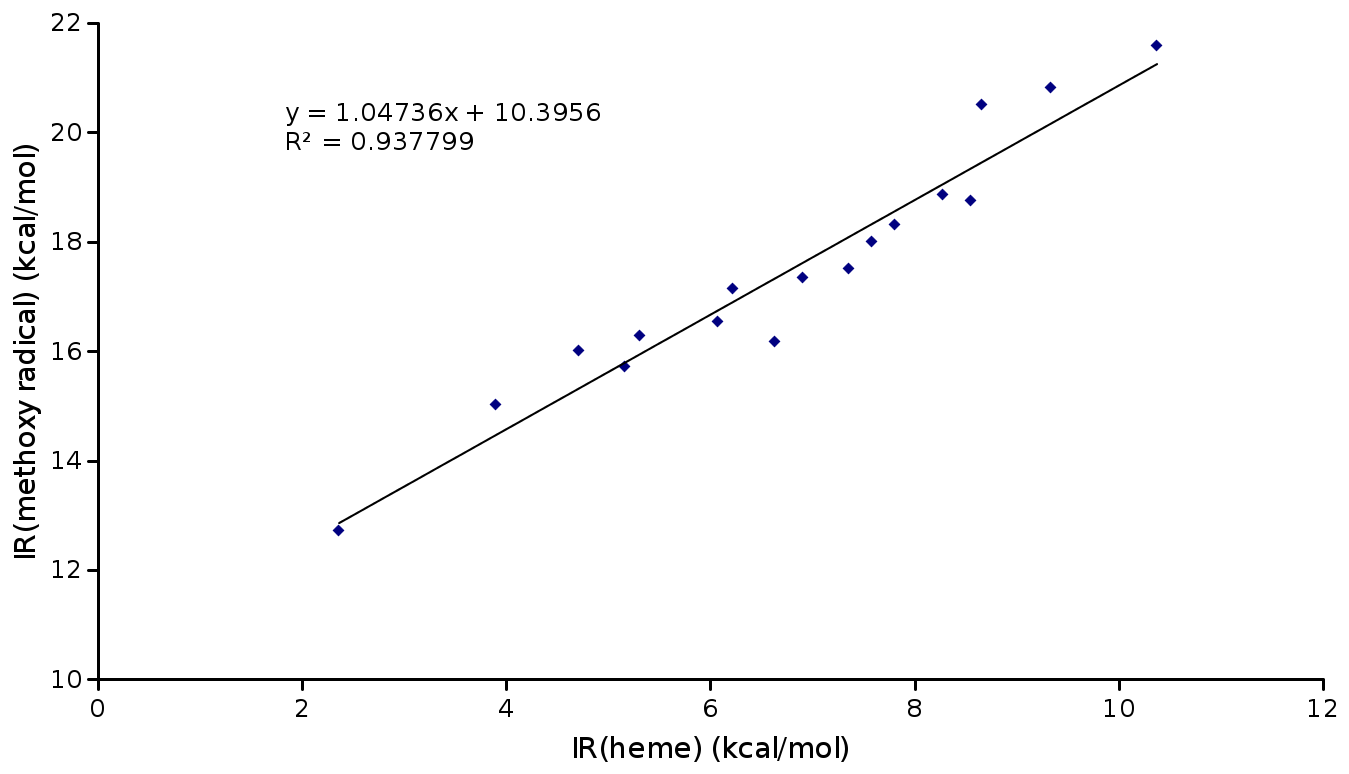
\includegraphics[width=0.8\textwidth]{figures/idsite/intrinsic_corrected.png}
\label{fig:idsite/intrinsic}
\caption{The linear relationship between the calculated intrinsic reactivity of the methoxy radical complex and that of the heme complex.
Adapted from \protect\cite{li2011idsite} with minor correction.
In the original manuscript the slope of the regression was reported as 1.117 and that number was used throughout.
This difference should not significantly affect the physical IDSite classifier results, and does not affect the results of the fit model.
In the rest of this text the value from the original publication of 1.117 will be used.}
\end{figure}
\begin{table}[h]
\centering
\label{table:heme_methoxy}
\begin{tabular}{cccc}
\hline
Model compound & Site of Metabolism & Heme model (kcal/mol) & Methoxy model (kcal/mol) \\
\hline
Benzene &  & 20.51 & 8.66 \\
Anisole & Ortho- & 16.29 & 5.31 \\
 & Meta- & 18.76 & 8.55 \\
 & Para- & 16.01 & 4.71 \\
 & Beta- & 16.18 & 6.63 \\
Dimethylether &  & 15.03 & 3.9 \\
Dimethylanisole & Meta- & 16.54 & 6.07 \\
 & Para- & 17.51 & 7.35 \\
Ethane &  & 21.58 & 10.37 \\
Ethanol & 1 & 12.73 & 2.36 \\
 & 2 & 17.35 & 6.9 \\
Propane &  & 18.31 & 7.8 \\
Toluene & Ortho- & 17.15 & 6.22 \\
 & Meta- & 18.86 & 8.27 \\
 & Para- & 18 & 7.58 \\
 & Alpha- & 15.72 & 5.16 \\
t-Butylebenzene & Beta- & 20.82 & 9.33 \\
\hline
\end{tabular}
\caption{DFT calculated values for internal reactivity of various compounds with either methoxy radical (compound I) or heme system.
Correlation between these values is illustrated in Figure \ref{fig:idsite/intrinsic}.}
\end{table}

\begin{equation}
\mathrm{IR}(\mathrm{heme}) = 1.117 * \mathrm{IR}(\mathrm{methoxy\ radical}) + C
\end{equation}
 % estimate from abbreviated reactivity
Since this constant $C$ is identical for each state it has no effect on the relative differences in ${\Delta}G_{\mathrm{site}}$ or the relative rate of metabolism at possible sites.
\begin{equation}
\label{equation:g_site}
E = \langle 1.117 * \mathrm{IR}(\mathrm{methoxyradical}) + C + E_{\mathrm{TS}} \rangle - kT\ ln(N_H)
\end{equation}
 % E/G equation
Since the ligand is forced to assume a different conformation in order to react, the energy of this transition state conformation, $E_{\mathrm{TS}}$, is also computed using PLOP.
As the relative abundance of different metabolites is determined by differences in ${\Delta}G$ per site rather than absolute reactivities, the constant in equation \ref{equation:g_site} does not affect which metabolites are produced.
A site of possible metabolism is classified as positive if it is observed in greater than 0.1\% yield, which corresponds to a \ddg\ of \textapprox4.75 kcal/mol between the most favored state and the cutoff for negative predictions. 

The second classifier is similar however:
\begin{enumerate}
\item a different constant is used to estimate $IR(\mathrm{heme})$ from $IR(\mathrm{methoxy\ radical})$, namely 1.071,
\item if the binding energy of the transition state complex of a pose is within 5.26 kcal/mol of the lowest pose, it is set to the binding energy of the lowest pose.
Otherwise the difference is scaled by 0.58,
\item and the cutoff for an active prediction is changed from 4.75 kcal/mol to 1.46 kcal/mol.
\end{enumerate}
These parameters were decided upon by maximizing $\frac{\mathrm{true\ positives}}{(\mathrm{false\ positives + false\ negatives})}$ on a training set of 36 compounds.

